\documentclass[11pt,graphicx,caption,rotating]{article}
\textheight=24cm
\textwidth=18cm
\topmargin=-2cm
\oddsidemargin=0cm
\usepackage[utf8x]{inputenc}
\usepackage[activeacute,spanish]{babel}
\usepackage{amssymb,amsfonts}
\usepackage[tbtags]{amsmath}
%\usepackage{slashbox}
\usepackage{pict2e}
\usepackage{float}
\usepackage[all]{xy}
\usepackage{graphics,graphicx,color,colortbl}
\usepackage{times}
\usepackage{subfigure}
\usepackage{wrapfig}
\usepackage{multicol}
\usepackage{cite}
\usepackage{url}
\usepackage[tbtags]{amsmath}
\usepackage{amsmath,amssymb,amsfonts,amsbsy}
\usepackage{bm}
\usepackage{algorithm}
\usepackage{algorithmic}
\usepackage[centerlast, small]{caption}
\usepackage[colorlinks=true, citecolor=blue, linkcolor=blue, urlcolor=blue,breaklinks=true]{hyperref}

\begin{document}
\begin{titlepage}
\begin{center}
{\huge \textbf{Bitácora De Laboratorio De Electrónica Análoga II}}\\[6cm]
{\Large \textbf{Elaborado por:}}\\
{\Large David Ricardo Martínez Hernández Código: $261931$}\\
{\Large José Duarte Código: $xxxxxx$, Mechudo}\\
{\Large Camilo Cadena Código: $xxxxxx$, Gomelo}\\[7cm]
{\Large \textbf{Electrónica Análoga II}}\\[6cm]
{\Large Universidad Nacional de Colombia}\\
{\Large Facultad de Ingeniería}\\
{\Large Bogotá}\\
{\Large 2012}\\
\date{}
\end{center}
\end{titlepage}
\tableofcontents
\listoftables
\listoffigures

\newpage

\floatname{algorithm}{Algoritmo}

\section{Guía 1: Amplificadores Simples con BJT}
\noindent
Dado que la polarización del transistor se encuentra en el archivo adjunto llamado \textit{Prinforme1.doc}, por consiguiente no se muestra que procedimiento se utilizo para caracterizar dichas configuraciones. Para cada configuración se realizo un programa en Matlab para calcular las ganancias, las impedancias tanto de entrada como de salida.\\
Los valores obtenidos en la práctica fueron los siguientes Cuadro \ref{tab1}:
\begin{table}[H]
	\centering
\begin{tabular}[c]{|c||c|c|} \hline
Elemento & Valor Nominal & Valor Medido \\ \hline
$R_1$ & $13$ K$\Omega$ & $13.003$ K$\Omega$ \\ \hline
$R_2$ & $62$ K$\Omega$ & $61.52$ K$\Omega$ \\ \hline
$R_C$ & $2.2$ K$\Omega$ & $2.225$ K$\Omega$ \\ \hline
$R_E$ & $0.56$ K$\Omega$ & $0.5136$ K$\Omega$ \\ \hline
\end{tabular}
	\caption{Tabla de valores tomados para las resistencias}
	\label{tab1}
\end{table}
\noindent
Los valores de operación del transistor fueron los siguientes
\begin{table}[H]
	\centering
\begin{tabular}[c]{|c||c|c|c|} \hline
 & Voltaje Teórico & Voltaje Práctico & \textbf{Error} \\ \hline
$V_E$ & $1.132$ V & $1.375$ V & $21\%$ \\ \hline
$V_B$ & $2.08$ V & $2.025$ V & $2.64\%$ \\ \hline
$V_C$ & $7.5494$ V & $7.01$ V & $7.14\%$ \\ \hline
$V_{CE}$ & $6.4124$ V & $5.653$ V & $7.63\%$ \\ \hline
\end{tabular}
	\caption{Tabla de valores tomados para el amplificador en polarización}
	\label{tab2}
\end{table}

\subsection{Amplificador de Emisor Común}
\noindent
Para determinar la ganancia de esta configuración se realizo un programa llamado \textit{emisor$\_$BJT.m}, este programa esta diseñado para determinar la ganancia para cualquier valor de resistencias, voltaje Colector-Emisor, Voltaje Early, Corriente de polarización y todos los factores que son necesarios para dicho análisis.
\begin{table}[H]
	\centering
\begin{tabular}[c]{|c|c|c|c|} \hline
$V_{IN}$ & $V_{OUT}$ & \textbf{Ganancia Práctica} V/V & \textbf{Error en la ganancia} \\ \hline
$8.64$ mV$_{RMS}$ & $1.02$ V$_{RMS}$ & $-118.056$ & $1.64\%$ \\ \hline
$8.94$ mV$_{RMS}$ & $1.07$ V$_{RMS}$ & $-119.687$ & $3.04\%$ \\ \hline
$9.53$ mV$_{RMS}$ & $1.13$ V$_{RMS}$ & $-118.573$ & $2.08\%$ \\ \hline
\end{tabular}
	\caption{Tabla de ganancias para la configuración a pequeña señal Emisor Común}
	\label{tab3}
\end{table}
\noindent
Para efectuar las mediciones se alimento el circuito con una señal sinodal de $10$ kHz de frecuencia de una amplitud de $20$mV (el límite de pequeña señal). La medida tomada en un osciloscopio analógico presentaba un voltaje pico de $2.22$ V y además presentaba un desfase de $180°$ correspondiente a medio periodo.\\
La ganancia teórica fue de $-116.148$ V/V. El error puede deberse a múltiples factores como la incertidumbre de los valores nominales de los componentes, variaciones en el beta del transistor, señales de distorsión debidas al generador de señales e interferencia al realizar las mediciones correspondientes.\\
El límite de la banda media (magnitud de $1.13$ V$*1/ \sqrt{3}=0.798$ V)  a una frecuencia de $375.4$ Hz, por debajo de la frecuencia medida inicialmente, al subir la frecuencia no varío la magnitud de la salida con las frecuencias que daba el generador.\\
El siguiente paso en este laboratorio consistió en modificar la configuración eliminando el condensador de desacople presente en el emisor, dando origen a una configuración conocida como emisor degenerado.Al desconectar el condensador de desacople de $47\ \ \mu$F y al aumentar la entrada se observo que la señal no se amplificaba mucho (Cuadro \ref{tab4})
\begin{table}[H]
	\centering
\begin{tabular}[c]{|c|c|c|} \hline
$V_{IN}$ & $V_{OUT}$ & \textbf{Ganancia Práctica} V/V \\ \hline
$42.7$ mV$_{RMS}$ & $109$ mV$_{RMS}$ & $-2.55269$ \\ \hline
\end{tabular}
	\caption{Tabla de valores tomados para la configuración en pequeña señal sin el condensador de desacople}
	\label{tab4}
\end{table}
\noindent
La impedancia de entrada del amplificador fue de $2.39266$ K$\Omega$. La inversión de fase se debe a que al aumentar la tensión de base, disminuye la tensión de salida, al disminuir la tensión de base, aumenta la tensión de salida, además la fuente de corriente establecida por el modelo de transconductancia la fuente de corriente dependiente se encuentra en sentido opuesto a la salida de tensión, esto genera la inversión de fase.\\
Al desconectar el condensador de desacoplo de emisor sucedió una caída de tensión, esto se debe a que se perdió la configuración de amplificador de emisor común y se transformo en un amplificador con degeneración.

\subsection{Amplificador Base Común}
\noindent
Para determinar la ganancia de esta configuración se realizo un programa llamado \textit{base$\_$BJT.m}, este programa esta diseñado para determinar la ganancia para cualquier valor de resistencias, voltaje Colector-Emisor, Voltaje Early, Corriente de polarización y todos los factores que son necesarios para dicho análisis.
\begin{table}[H]
	\centering
\begin{tabular}[c]{|c|c|c|c|} \hline
$V_{IN}$ & $V_{OUT}$ & \textbf{Ganancia Práctica} V/V & \textbf{Error en la ganancia} \\ \hline
$10.1$ mV$_{RMS}$ & $50.05$ mV$_{RMS}$ & $25.50$ & $6\%$ \\
 \hline
\end{tabular}
	\caption{Tabla de ganancias para la configuración a pequeña señal Base Común}
	\label{tab5}
\end{table}
\noindent
Siendo la ganancia teórica de $24.06$ V/V.\\
Para $462$ mV de entrada dan $446$ mV de salida a $10$ kHz.\\
Al desconectar el condensador de desacople de $47\ \mu$F y al aumentar la entrada se cae el voltaje porque la configuración del transistor ha cambiado y se transformó en una configuración con degeneración.\\
La impedancia de entrada del amplificador fue de $61.11$ $\Omega$. La inversión de fase se debe al mismo fenómeno que sucede en el amplificador de emisor común.\\

\subsection{Amplificador Colector Común}
Para determinar la ganancia de esta configuración se realizo un programa llamado \textit{colector$\_$BJT.m}, este programa esta diseñado para determinar la ganancia para cualquier valor de resistencias, voltaje Colector-Emisor, Voltaje Early, Corriente de polarización y todos los factores que son necesarios para dicho análisis.
\begin{table}[H]
	\centering
\begin{tabular}[c]{|c|c|c|c|} \hline
$V_{IN}$ & $V_{OUT}$ & \textbf{Ganancia Práctica V/V} & \textbf{Error en la ganancia} \\ \hline
$20$ mV$_{RMS}$ & $17$ V$_{RMS}$ & $0.946$ & $3\%$ \\ \hline
\end{tabular}
	\caption{Tabla de ganancias para la configuración a pequeña señal Colector Común}
	\label{tab6}
\end{table}
\noindent
Siendo la ganancia teórica de $0.976$ V/V.\\
El límite de la banda media (magnitud de $1.13$ V$*1/ \sqrt{3}=0.798$ V)  a una frecuencia de $375.4$ Hz, por debajo de la frecuencia medida inicialmente, al subir la frecuencia no varío la magnitud de la salida con las frecuencias que daba el generador.\\
La impedancia de entrada del amplificador fue de $9.89$ K$\Omega$. No hay inversión de fase en el amplificador de colector común.

\subsection{Conclusiones}
\begin{itemize}
 \item Se conocieron las diferentes configuraciones para los BJT's, como lo es el emisor común que se utiliza para obtener ganancia de voltaje, el colector común que se utiliza para ganancia de corriente con una impedancia de entrada muy baja y para acople de impedancias, y finalmente el base común que se utiliza para amplificación de voltaje un poco más pequeña que el emisor común pero su ancho de banda es mas elevado.
 \item Las impedancias de cada amplificador son aprovechadas para realizar conexiones en cascada y así .
\end{itemize}

\section{Guía 2: Caracterización de Transistores de Efecto de Campo y Amplificadores Básicos}
\noindent
Dado que la polarización del transistor se encuentra en el archivo adjunto llamado \textit{Prinforme2doc}, por consiguiente no se muestra que procedimiento se utilizo para caracterizar dichas configuraciones. Para cada configuración se realizo un programa en Matlab para calcular las ganancias, las impedancias tanto de entrada como de salida.\\
Los valores obtenidos en la práctica fueron los siguientes Cuadro \ref{tab10}:

\begin{table}[H]
	\centering
\begin{tabular}[c]{|c||c|c|} \hline
Elemento & Valor Nominal & Valor Medido \\ \hline
$R_1$ & $470$ K$\Omega$ & $468.6$ K$\Omega$ \\ \hline
$R_2$ & $560$ K$\Omega$ & $571.6$ K$\Omega$ \\ \hline
$R_D$ & $2.2$ K$\Omega$ & $2.189$ K$\Omega$ \\ \hline
$R_S$ & $0.33$ K$\Omega$ & $0.331$ K$\Omega$ \\ \hline
\end{tabular}
	\caption{Tabla de valores tomados para las resistencias}
	\label{tab7}
\end{table}

\subsection{Canal N}
\noindent
Dado el montaje de la Guía $2$ (Figura 2) es el más adecuado para poder medir el voltaje de encendido \textit{Vt}, dado que garantiza que la corriente de Drenador sea $0$, esto asegura que $Vd=Vg$, tal que:
\begin{equation}
 I_{D}=kn (Vgs-Vt)^{2}=0
\label{ecu1}
\end{equation}
\noindent
Como la transconductancia es diferente de $0$, la condición quedaría como
\begin{equation}
 V_{gs}=V_t=V_d
\label{ecu2}
\end{equation}
\noindent
como aún no he se ha verificado la hipótesis en la que el transistor se encuentra en saturación, es decir
\begin{equation}
 V_{ds} \geq V_{gs}-V_t
\label{ecu3}
\end{equation}
\noindent
Para poder medir el parámetro $k_n$ puede ser fácilmente medido, tomando $V_{gs}=V_d$ y se puede determinar $i_d$ por medio de
\begin{equation}
 i_d=\frac{V_{dd}-V_d}{R}
\label{ecu4}
\end{equation}
\noindent
Finalmente para determinar el valor de $k_n$ se reemplaza dicha expresión en la ecuación de Shockley dando como resultado
\begin{equation}
 k_n=\frac{V_{dd}-V_d}{R(V_d-V_t)^{2}}
\end{equation}

\subsection{Canal P}
\noindent
Dado el montaje de la Guía $2$ (Figura 3) es el más adecuado para poder medir el voltaje de encendido \textit{Vt}, dado que garantiza que la corriente de Drenador sea $0$, esto asegura que
\begin{equation}
 V_{sg}=|V_t|
\label{ecu5}
\end{equation}
\noindent
El signo de $V_t$ depende de la naturaleza del dispositivo. Al igual que la demostración del canal N se puede asumir que el transistor se encuentra trabajando en saturación, es decir
\begin{equation}
 V_{sd} \leq V_{sg}-|V_t|
\label{ecu6}
\end{equation}
\noindent
Para determinar el valor de $k_p$, se inicia de la ecuación de Shockley para dispositivos de canal P
\begin{equation}
 i_d=kp(V_{sg}-V_t)^2
\label{ecu7}
\end{equation}
Además
\begin{equation}
 V_{sg}=V_{dd}-V_d
\label{ecu8}
\end{equation}
\begin{equation}
 i_d=\frac{V_d}{R}
\label{ecu9}
\end{equation}
\noindent
Despejando de la ecu (\ref{ecu7}) y reemplazando se obtiene:
\begin{equation}
 k_p=\frac{i_d}{(V_{sg}-|V_t|)^{2}}=\frac{V_d}{R(V_{sg}-|V_t|)^{2}}
\label{ecu10}
\end{equation}

\subsection{Caracterización de Transistores de Efecto de Campo}
\subsubsection{Canal N}
\begin{table}[H]
	\centering
\begin{tabular}[c]{|c|c|c|c|} \hline
Transistores & $V_{dd}$ & $V_d$ & $V_t$ \\ \hline
$3,4,5$ & $14.96$ V & $14.72$ V & $0.24$ V \\ \hline
$6,7,8$ & $14.96$ V & $14.70$ V & $0.26$ V \\ \hline
$9.10.11$ & $14.96$ V & $14.71$ V & $0.25\%$ V \\ \hline
\end{tabular}
	\caption{Valores de $V_t$ para los transistores de canal N}
	\label{tab8}
\end{table}
\begin{table}[H]
	\centering
\begin{tabular}[c]{|c|c|c|c|} \hline
Transistores & $V_{dd}$ & $V_d$ & $k_n$ \\ \hline
$3,4,5$ & $14.96$ V & $8.09$ V & $0.113068$ \\ \hline
$6,7,8$ & $14.96$ V & $14.70$ V & $0.113191$ \\ \hline
$9.10.11$ & $14.96$ V & $14.71$ V & $0.115189$ \\ \hline
\end{tabular}
	\caption{Valores de $k_n$ para los transistores de canal N para una resistencia de $0.986$ k$\Omega$}
	\label{tab9}
\end{table}

\subsubsection{Canal P}
\begin{table}[H]
	\centering
\begin{tabular}[c]{|c|c|c|c|} \hline
Transistores & $V_{dd}$ & $V_d$ & $V_t$ \\ \hline
$1,2,3$ & $12.02$ V & $10.51$ V & $1.51$ V \\ \hline
$10,11,12$ & $12.02$ V & $10.53$ V & $1.49$ V \\ \hline
$13,14,6$ & $12.02$ V & $10.52$ V & $1.5\%$ V \\ \hline
\end{tabular}
	\caption{Valores de $V_t$ para los transistores de canal P}
	\label{tab10}
\end{table}
\begin{table}[H]
	\centering
\begin{tabular}[c]{|c|c|c|c|} \hline
Transistores & $V_{dd}$ & $V_d$ & $k_n$ \\ \hline
$1,2,3$ & $12.02$ V & $5.83$ V & $0.271059$ \\ \hline
$10,11,12$ & $12.02$ V & $5.80$ V & $0.263.994$ \\ \hline
$13,14,6$ & $12.02$ V & $14.71$ V & $0.268296$ \\ \hline
\end{tabular}
	\caption{Valores de $k_p$ para los transistores de canal N para una resistencia de $0.982$ k$\Omega$}
	\label{tab11}
\end{table}

\subsection{Amplificador de Fuente Común}
\noindent
Para determinar la ganancia de esta configuración se realizo un programa llamado \textit{source$\_$FET.m}, este programa esta diseñado para determinar la ganancia para cualquier valor de resistencias, voltaje Drain-Source, Voltaje Early, Corriente de polarización y todos los factores que son necesarios para dicho análisis.
\begin{table}[H]
	\centering
\begin{tabular}[c]{|c|c|c|c|} \hline
\textbf{Ganancia Práctica} V/V & \textbf{Error en la ganancia} \\ \hline
$2.5$ & $4.52\%$ \\ \hline
\end{tabular}
	\caption{Tabla de ganancias para la configuración a pequeña señal Fuente Común}
	\label{tab12}
\end{table}
\noindent
Siendo la ganancia teórica de .\\
El error puede deberse a múltiples factores como la incertidumbre de los valores nominales de los componentes, variaciones en el beta del transistor, señales de distorsión debidas al generador de señales e interferencia al realizar las mediciones correspondientes.\\
La frecuencia de corte fue de $f_c=950$ kHz. Al aproximarse a la frecuencia de corte la ganancia empieza a disminuir por que el transistor comienza a recortar la señal por el ancho de banda de dicha configuración, no se puede exceder este limite dado que es un elemento real, además a esta frecuencia tiene otro tipo de operación el cual no conocemos. \\
Relación de impedancias.

\subsection{Amplificador de Compuerta Común}
\noindent
Para determinar la ganancia de esta configuración se realizo un programa llamado \textit{gate$\_$FET.m}, este programa esta diseñado para determinar la ganancia para cualquier valor de resistencias, voltaje Drain-Source, Voltaje Early, Corriente de polarización y todos los factores que son necesarios para dicho análisis.
\begin{table}[H]
	\centering
\begin{tabular}[c]{|c|c|} \hline
\textbf{Ganancia Práctica} V/V & \textbf{Error en la ganancia} \\ \hline
$2.5$ & $4.98\%$ \\ \hline
\end{tabular}
	\caption{Tabla de ganancias para la configuración a pequeña señal Compuerta Común}
	\label{tab13}
\end{table}
\noindent
Siendo la ganancia teórica de .\\
Para darle una explicación al error se llego a la conclusión que fue causado por los mismos problemas que en la configuración de Fuente común.\\
La frecuencia de corte fue de $f_c=575$ kHz.\\
Relación de impedancias

\subsection{Amplificador de Drain Común}
\noindent
Para determinar la ganancia de esta configuración se realizo un programa llamado \textit{drain$\_$FET.m}, este programa esta diseñado para determinar la ganancia para cualquier valor de resistencias, voltaje Drain-Source, Voltaje Early, Corriente de polarización y todos los factores que son necesarios para dicho análisis.
\begin{table}[H]
	\centering
\begin{tabular}[c]{|c|c|c|} \hline
\textbf{Ganancia Práctica} V/V & \textbf{Error en la ganancia} \\ \hline
$2.5$ & $4.01\%$ \\ \hline
\end{tabular}
	\caption{Tabla de ganancias para la configuración a pequeña señal Drain Común}
	\label{tab14}
\end{table}
\noindent
Siendo la ganancia teórica de .\\
Para darle una explicación al error se llego a la conclusión que fue causado por los mismos problemas que en la configuración de Fuente común.\\
La frecuencia de corte fue de $f_c=1.35$ MHz.\\
Relación de impedancias

\section{Guía 3: Fuentes y Espejos de Corriente}
\noindent
Dado que la polarización del transistor se encuentra en el archivo adjunto llamado \textit{Prinforme3.doc}, por consiguiente no se muestra que procedimiento se utilizo para caracterizar dichas configuraciones. Para cada configuración se realizo un programa en Matlab para calcular las ganancias, las impedancias tanto de entrada como de salida, el archivo se llama \textit{Simple$\_$Mirror.m}.\\
Su respectivo informe se encuentra adjunto en el archivo \textit{Práctica 3}.

\section{Guía 4: Fuente de corriente con MOSFET y amplificador diferencial BJT}
\noindent
Dado que la polarización del transistor se encuentra en el archivo adjunto llamado \textit{Prinforme4.doc}, por consiguiente no se muestra que procedimiento se utilizo para caracterizar dichas configuraciones. Para cada configuración se realizo un programa en Matlab para calcular las ganancias, las impedancias tanto de entrada como de salida.\\
Los valores obtenidos en la práctica fueron los siguientes Cuadro \ref{tab1}:
\begin{table}[H]
	\centering
\begin{tabular}[c]{|c||c|c|} \hline
Elemento & Valor Nominal & Valor Medido \\ \hline
$R_1$ & $13$ K$\Omega$ & $13.003$ K$\Omega$ \\ \hline
$R_2$ & $62$ K$\Omega$ & $61.52$ K$\Omega$ \\ \hline
$R_C$ & $2.2$ K$\Omega$ & $2.225$ K$\Omega$ \\ \hline
$R_E$ & $0.56$ K$\Omega$ & $0.5136$ K$\Omega$ \\ \hline
\end{tabular}
	\caption{Tabla de valores tomados para las resistencias}
	\label{tab15}
\end{table}
\noindent
Los valores de operación del transistor fueron los siguientes
\begin{table}[H]
	\centering
\begin{tabular}[c]{|c||c|c|c|} \hline
$R_L$ k$\Omega$ & $V_{R_{L}}$ & $I_{R_{L}}$ mA & $V_{DS}$ V \\ \hline
$0.1011$ & $0.212$ & $2.0969$ & $11.71$ \\ \hline
$0.5215$ & $1.089$ & $2.0882$ & $10.83$ \\ \hline
$0.986$ & $2.043$ & $2.07200$ & $9.87$ \\ \hline
$1.792$ & $3.699$ & $2.06417$ & $8.22$ \\ \hline
$2.139$ & $4.404$ & $2.04952$ & $7.51$ \\ \hline
$3.796$ & $7.78$ & $2.05890$ & $4.124$ \\ \hline
$4.621$ & $9.23$ & $1.99740$ & $2.68$ \\ \hline
$5.4868$ & $10.5$ & $1.91368$ & $1.411$ \\ \hline
$9.75$ & $11.4$ & $1.16923$ & $0.515$ \\ \hline
\end{tabular}
	\caption{Tabla de valores tomados para el espejo de corriente en polarización}
	\label{tab16}
\end{table}
\noindent
En base a la figura \ref{fig3} se asegura que la potencia máxima disipada por el transistor
ocurre cuando la resistencia de carga es mínima.

\subsection{Espejo de Corriente Simple con MOSFET}
\noindent

\begin{figure}[H]
	\centering
		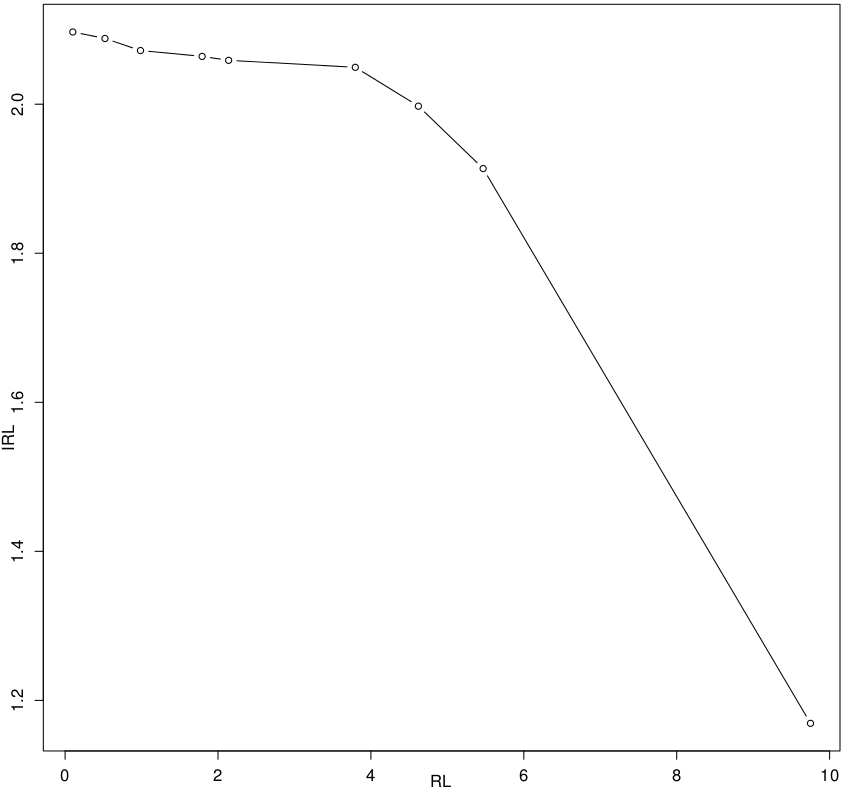
\includegraphics[scale=0.5]{corriR.png}
	\caption{Gráfica de Resistencia en función de la corriente}
	\label{fig1}
\end{figure}
\begin{figure}[H]
	\centering
		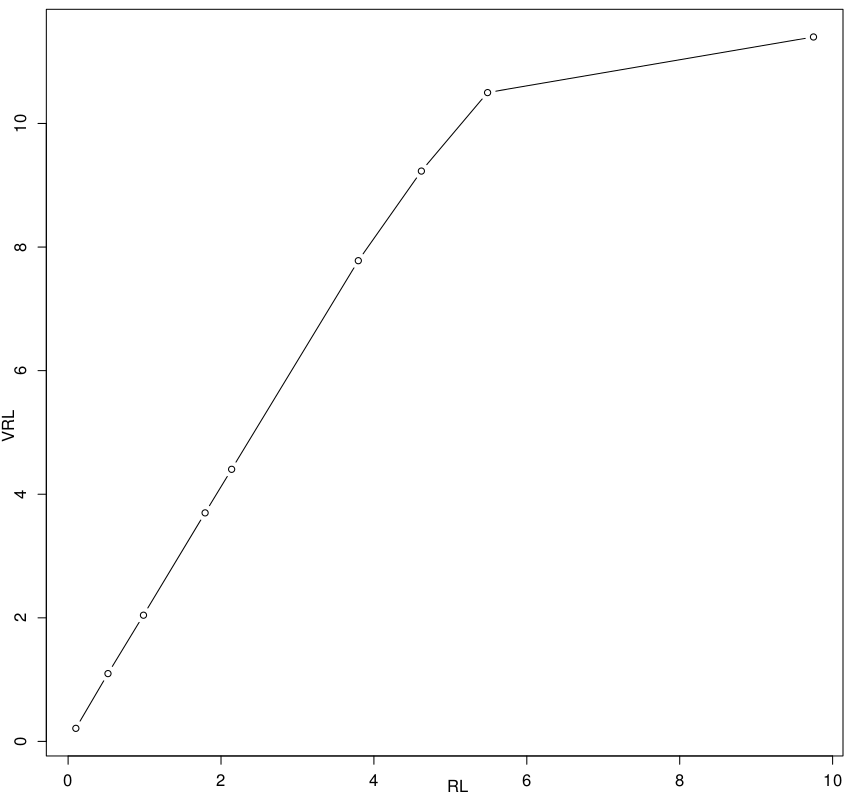
\includegraphics[scale=0.5]{voltR.png}
	\caption{Gráfica de Resistencia en función del voltaje}
	\label{fig2}
\end{figure}
\begin{figure}[H]
	\centering
		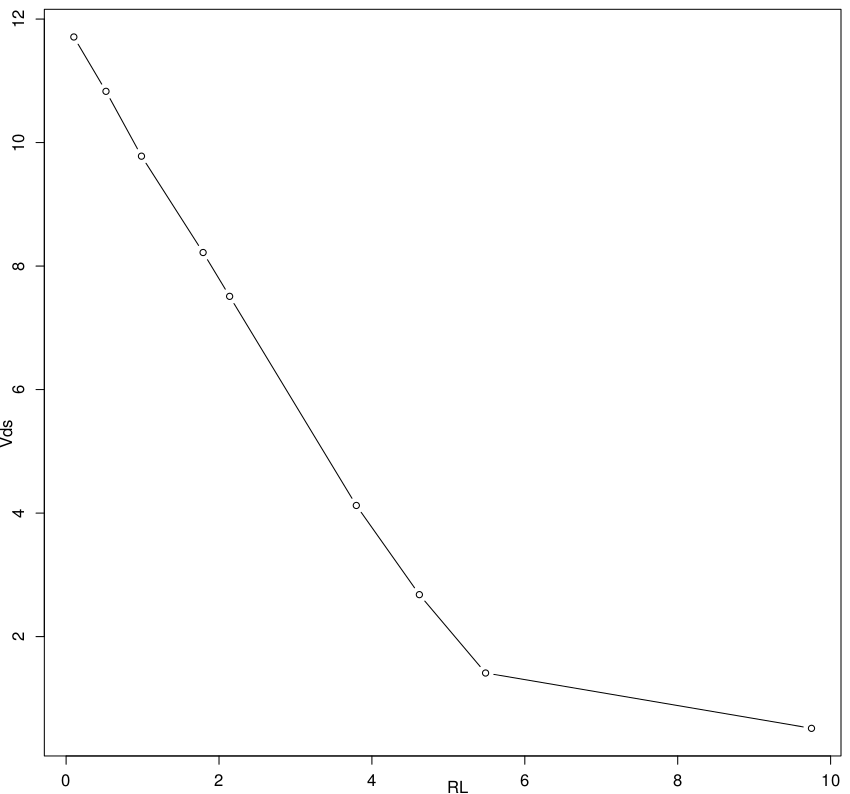
\includegraphics[scale=0.5]{vdsR.png}
	\caption{Gráfica de Resistencia en función del voltaje Drane-Source}
	\label{fig3}
\end{figure}

\subsection{Amplificador Diferencial BJT con carga resistiva}
\noindent
Para el amplificador diferencial con carga resistiva y cola resistiva se diseño un programa llamado \textit{Differential$\_$Ampllificator.m}.\\
Los datos de polarización son los siguientes
\begin{table}[H]
	\centering
\begin{tabular}[c]{|c|c||c|c|} \hline
$R_{C1}$ & $5.52$ & $V_{CC}$ & $14.90$ \\ \hline
$R_{B1}$ & $16.3$ & $V_{CE_{3}}$ & $4.45$ \\ \hline
$R_{C2}$ & $5.52$ & $V_{CE_{1}}$ & $9.87$ \\ \hline
$R_{B2}$ & $16.15$ & $V_{CE_{2}}$ & $8.22$ \\ \hline
$R_{E}$ & $1.47$ & $V_{C_{1}}$ & $7.51$ \\ \hline
$R_{Z}$ & $19.6$ & $V_{C_{2}}$ & $4.124$ \\ \hline
$R_{L}$ & $0.2347$ & $V_{E_{3}}$ & $2.68$ \\ \hline
$I_{C_{1}}$ & $1.3677$ & $I_{C_{2}}$ & $1.50362$ \\ \hline
\end{tabular}
	\caption{Tabla de valores tomados para el amplificador diferencial con Carga Resistiva en polarización}
	\label{tab17}
\end{table}
\noindent
La corriente obtenida a partir de la fuente fue de $2.997$ mA.\\
\begin{table}[H]
	\centering
\begin{tabular}[c]{|c|c|c|} \hline
 & Ganancia Práctica & Error \\ \hline
Ganancia Diferencial & $97$ & $3.5\%$ \\ \hline
Ganancia Modo Común & $-0.00194$ & $3\%$ \\ \hline
\end{tabular}
	\caption{Tabla de valores tomados para el Amplificador Diferencial con Carga Resistiva a pequeña señal}
	\label{tab18}
\end{table}
\noindent
El valor del CMRR fue de $93.706$ dB.\\
El error se debe a que el calculo de la resistencia Norton de la fuente zener no fue hecho con los valores de la corriente, voltaje Early y beta reales del transistor, por el contrario se hizo con los considerados en la hoja de datos.

\subsection{Amplificador Diferencial con Cola Resistiva}
\noindent
Los valores obtenidos en esta parte fueron muy similares, lo que vario fue la ganancia al modo diferencial y al modo común.
\begin{table}[H]
	\centering
\begin{tabular}[c]{|c|c|c|} \hline
 & Ganancia Práctica & Error \\ \hline
Ganancia Diferencial & $96$ & $3.8\%$ \\ \hline
Ganancia Modo Común & $-0.6545$ & $3\%$ \\ \hline
\end{tabular}
	\caption{Tabla de valores tomados para el Amplificador Diferencial con Cola Resistiva a pequeña señal}
	\label{tab19}
\end{table}
\noindent
El valor del CMRR fue de $43.381$ dB.\\
dados los resultados obtenidos en la práctica al aumentar tener una ganancia menor al modo común se obtiene una mejor señal de salida, esto se puede comprobar al agregar una cola resistiva al diferencial o un carga resistiva.

\section{Guía 7: Amplificadores Operacionales}
\noindent
El preinforme de esta práctica se encuentra en el archivo adjunto llamado, \textit{preinforme7.doc}, además se realizó un programa en Matlab llamado \textit{OpAm.m}, el cual permite determinar la ganancia para cualquier valor de resistencias.

\subsection{Seguidor de tensión}
\begin{table}[H]
	\centering
\begin{tabular}[c]{|c|c|} \hline
 Ganancia Práctica & Error \\ \hline
$V_{CC}$ V & $V_S$ V \\ \hline
$1.7$ & $1.7$ \\ \hline
$5.4$ & $5.41$ \\ \hline
$7.8$ & $7.8$ \\ \hline
$9.01$ & $9$ \\ \hline
$14.25$ & $14.25$ \\ \hline
$22.8$ & $22.81$ \\ \hline
\end{tabular}
	\caption{Tabla de valores tomados para el Seguidor de tensión}
	\label{tab20}
\end{table}
\noindent
El ancho de banda de este seguidor es de: $62$ kH.\\
La variación que existe entre la salida y la entrada es muy similar, loas variaciones de la entrada se ven reflejados en la señal de salida. Por otro lado se observo la respuesta del seguidor a la variación de frecuencia. Dados los resultados se puede concluir que el seguidor de tensión posee un ancho de banda aceptable ṕor su gran respuesta a la variación de frecuencia, por otro lado es muy pequeño el ancho de banda coparado con el ancho de banda del seguidor por emisor


\subsection{Amplificador Inversor}
\noindent
En el amplificador inversor el ancho de banda fue de $144$ kHz.\\
En la práctica se implemento una relación de resistencia de $2$ a $1$ y $10$ a $1$ entre $R_2$ y $R_1$. Las ganancias que se habían calculado se aproximaban a los resultados experimentales con errores muy bajos. Sin embargo el ancho de banda es mayor en los amplificadores BJT.

\subsection{Sumador}
\noindent
En esta parte de la práctica se tomo una señal y primero se invirtio mediante un amplificador inversor de ganancia 1, con esta señal y la señal original se alimento un sumador basado en operacionales cuya salida fue de $0.4$ mV, muy cercana a $0$. Dado que la salida es mayor a $0$ quiere decir que se presento un error en la s ganancias, esto se debe a que no se utilizo el modelo real del operacional y la incertidumbre de las resistencias no se tomo en cuenta.


\section{Guía 5: Amplificador Mosfet con carga activa y Amplificadores Operacionales}
\noindent
Dado que la polarización del transistor se encuentra en el archivo adjunto llamado \textit{Prinforme5.doc}, por consiguiente no se muestra que procedimiento se utilizo para caracterizar dichas configuraciones. Para cada configuración se realizo un programa en Matlab para calcular las ganancias, las impedancias tanto de entrada como de salida, llamado \textit{reactivo.m}.\\

\subsection{Polarización por realimentación desde el Drenador}
\noindent
Esta parte del laboratorio no se pudo realizar dados los problemas presentados de polarización y los elementos de laboratorio no se encontraban en buenas condiciones, se dificulto dicha práctica.

\subsection{Derivador}
\noindent
Dado que el Integrador se puede construir con condensadores y bobinas dependiendo de la realimentación, aunque es mucho más sencillo realizarlo por medio de condensadores dado que tienen una respuesta al voltaje muy suave, esto hace que no sea tan brusca la respuesta, cuando se realiza con bobinas se encuentran sistemas de segundo orden, esto hace que se tenga una respuesta sobre-amortiguada, esto se debe a las capacitancias encontradas en la bobina.
\begin{figure}[H]
	\centering
		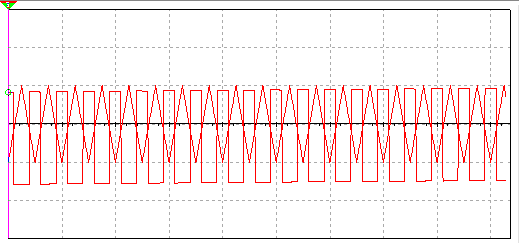
\includegraphics[scale=0.7]{derivador1.png}
	\caption{Simulación Derivador, señal triangular}
	\label{fig4}
\end{figure}
\begin{figure}[H]
	\centering
		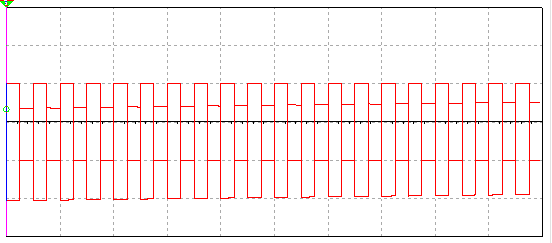
\includegraphics[scale=0.7]{derivador2.png}
	\caption{Simulación Derivador, señal cuadrada}
	\label{fig5}
\end{figure}

\subsection{Integrador}
\noindent
Dado que el Integrador se puede construir con condensadores y bobinas dependiendo de la realimentación, aunque es mucho más sencillo realizarlo por medio de condensadores dado que tienen una respuesta al voltaje muy suave, esto hace que no sea tan brusca la respuesta.
\begin{figure}[H]
	\centering
		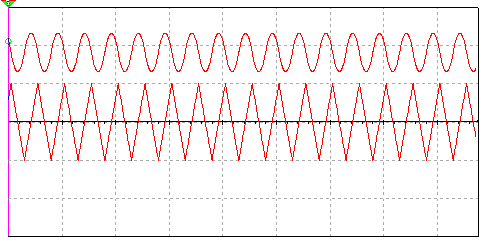
\includegraphics[scale=0.7]{integrador.png}
	\caption{Simulación Integrador, señal triangular}
	\label{fig6}
\end{figure}
\begin{figure}[H]
	\centering
		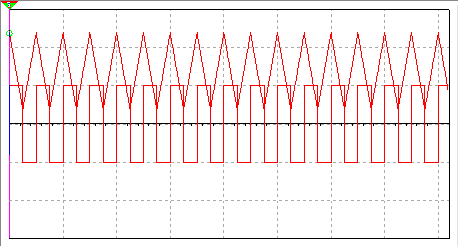
\includegraphics[scale=0.7]{integrador2.png}
	\caption{Simulación Integrador, señal Cuadrada}
	\label{fig6}
\end{figure}

\subsection{Amplificador No Inversor}
\noindent
En el laboratorio se utilizaron las resistencias correspondientes lo que genero que la señal de salida estuviera amplificada 10 veces más que la señal de entrada, con la misma fase.

\section{Guía 6: Amplificador Mosfet diferencial con carga activa}
\noindent
La polarización del amplificador se encuentra en un archivo adjunto llamado \textit{preinforme6.doc}, y también tiene un programa el cual calcula la ganancia para cualquier valor de resistencias llamado \textit{reactivo$\_$2.m}.\\
No se pudo realizar la práctica por los problemas presentados en el laboratorio, los elementos se encontraban en mal estado y no se pudo realizar, además el haber quemado el CI altero los resultados que se esperaban y toco nuevamente a caracterizarlo.

\bibliographystyle{ieeetran}
\begin{thebibliography}{99}
\bibitem{sedra} Jaeger, Richard C. \& Blalock, Travis N.
{\em "`Microelectronic Circuit Desing"'}.
McGraw-Hill, Fourth Edition, 1999.

\bibitem{sedra} Sedra, Adel S. \& Smith, Kenneth C.
{\em "`Circuitos Microelectrónicos"'}.
Oxford University Press, Cuarta Edición, 1999.
\end{thebibliography}
\end{document}